% !TEX encoding = MacOSRoman
\documentclass[handout]{beamer}
\usepackage[frenchb]{babel}
\usepackage[T1]{fontenc}
\usepackage[utf8]{inputenc}
\usepackage{graphicx}


% functions to plot
\def\func(#1){(#1)*(1-(#1))}
\hypersetup{colorlinks = true,linkcolor = blue,urlcolor  = blue}
            
\newcommand{\qGraph}[1]{\begin{center} \includegraphics[width =
\textwidth]{#1}\end{center}}

\newcommand{\mcl}{\mathcal}

\addtobeamertemplate{navigation symbols}{}{%
    \usebeamerfont{footline}%
    \usebeamercolor[fg]{footline}%
    \hspace{1em}%
    \insertframenumber/\inserttotalframenumber
}

\newenvironment{iPar}[1]{\textbf{#1} \begin{itemize}}{\end{itemize}}

\newcommand{\inc}{{inc}}
\newcommand{\cp}{{cmp}}
\newcommand{\bull}{$\bullet\;$} 

\newcommand{\esp}{\mathbf{E}} \newcommand{\ul}[1]{\underline{#1}}
\newcommand{\ol}[1]{\overline{#1}} \newcommand{\ora}[1]{\textbf{#1}}
\newcommand{\wh}{\widehat}
\newcommand{\mdp}{\medskip \pause}
\newcommand{\mc}{\mathcal}

\title{Choix avec Risque}
\author{Microéconomie \\ 20851}
\date{}

\begin{document}

\frame{\titlepage}

\section[Outline]{}
\frame{\tableofcontents}

\section{}


\begin{frame}\frametitle{Itinéraire}

\begin{iPar}{Jusqu'à maintenant}
\item Préférences consommateur
\item Choix du consommateur
\item Effets prix et revenu
\end{iPar}\mdp

\begin{iPar}{Ce cours: risque}
\item Pour comprendre les choix d'assurance et d'investissements
\end{iPar}\mdp

\begin{iPar}{Plus tard}
\item Intertemporel
\item Mesurer le bien-être
\item  Équilibre de marché en situation d'échange
\item  La production et le comportement stratégique des firmes
\item  Enchères
\end{iPar}
\end{frame}

\section{Les préférences}

\begin{frame}\frametitle{Préférences en contexte d'incertitude}

\begin{iPar}{Les gens n'aiment pas le risque en général}\item Revenu de retraite moyen: \$$50 \; 000$/an \item  Imaginez que vous épargnez pour la retraite:
Devez choisir entre (obligations, actions ...) \item Problème
1: \begin{tabular}{ll} \textbf{actif sans risque} & 50\; 000/an\\
\textbf{actif risqué} & 50\% chance  10 000/an \\ & 50\%  chance  90
000/an\end{tabular} \medskip \item Revenu moyen 50 000/an dans les deux cas, lequel choisissez vous? \end{iPar}

\end{frame}

\begin{frame}\frametitle{Arbitrage risque rendement}

\begin{iPar}{Trois problème de choix}
\item \begin{tabular}{lll} \textbf{Choix 1:} & \textbf{sans risque} & 50\; 000/an\\
&\textbf{risque} & 50\% chance  10\; 000/an \\& & 50\%  chance  90\; 000/an\end{tabular} \mdp \item \begin{tabular}{lll}\textbf{Choix 2:} &  \textbf{sans risque} & 50\; 000/an\\
& \textbf{risque} & 50\% chance  10\; 000/an \\ & & 50\%  chance  100\; 000/an\end{tabular} \mdp \item  \begin{tabular}{lll} \textbf{Choice 3:} & \textbf{sans risque} & 50\; 000/an\\
& \textbf{risque} & 50\% chance  10\; 000/an \\ &&  50\%  chance
110\; 000/an\end{tabular} \end{iPar} \end{frame}


\begin{frame}\frametitle{L'approche d'espérance d'utilité}

\begin{iPar}{Loterie et espérance d'utilité} 
\item Loterie $\mathcal L = (p,X \;; 1-p,Y)$ : avec
probabilité $p$ donne $X$, et probabilité $1-p$ donne $Y$ \item Espérance d'utilité $$
\mathbf \mathbb{E}_{{ \mathcal L}} (u) = p\times u(X) + (1-p) \times
u(Y)$$ \end{iPar}\mdp



\begin{iPar}{Préférences sur des loteries} \item Modèle: Consommateur préfère
loterie $\mathcal L_1$ à loterie $\mathcal L_2$ ssi $$\mathbf \mathbb
{E}_{{ \mathcal L_1}} (u) > \mathbf \mathbb{E}_{{ \mathcal L_2}} (u)$$
\item Note: utilité est cardinale (ses unités et forme sont importantes). Dénommé utilité \href{https://fr.wikipedia.org/wiki/John_von_Neumann}{von Neumann} et Morgenstern (vNM). 
\end{iPar}

\end{frame}

\begin{frame}{Exemple}

\begin{iPar}{Contexte} \item $u(X) = \sqrt{X}$ \item $\mathcal L_1 =
(0.5,0\;; 0.5,16)$ et $\mathcal L_2 = (1,6)$ \item \textbf{Exercice A}: Rendement espéré? \item
\textbf{Exercice B} Quel est le choix du consommateur ?  \item \textbf{Exercice C}: Est-ce que la fonction d'utilité $\tilde u(X) = X$ donne le même comportement?\end{iPar}

\end{frame}

\begin{frame}{Identifier les préférences à partir des choix}

\begin{iPar}{Préfèrences invariante à transformation affine}
\item Transformation affine: $\wh u = a u +b$ avec $a>0$
\begin{align*}
\esp_{L_1} \wh u \geq \esp_{L_2} \wh u & \iff  a\esp_{L_1} u + b \geq a\esp_{L_2} u + b \\ & \iff 
 \esp_{L_1} u  \geq \esp_{L_2} u
\end{align*}\mdp

\end{iPar}

\end{frame}

\section{Riscophobie et Riscophilie}

\begin{frame}\frametitle{Les consommateurs riscophobe and riscophile}
\begin{iPar}{Attitudes différentes au risque} \item Aversion au risque (riscophobe): considérons $L = (p, X\;; 1-p,Y)$\\
Si on dénote $Z = p X + (1-p)Y $. \mdp

consommateur est riscophobe s'il préfère $\mathcal L' = (1,Z)$ à $\mathcal L$  \mdp \item Riscophile: elle préfère $ \mathcal L = (p, X\;; 1-p,Y) $ à  $\mathcal L' =
(1,Z)$ \end{iPar}\mdp

\begin{iPar}{Qu'est-ce qu'on observe?} \item Un peu de comportement riscophile (casinos
... ) mais ne tient pas compte de la valeur de "l'expérience" \item  Beaucoup d'aversion au risque (assurance, épargne, investissement ...) \end{iPar} \end{frame}


\begin{frame}\frametitle{Aversion au risque et concavité de l'utilité}

\begin{iPar}{Aversion au risque} \item Consommateur a l'utilité $u$ \item Étant donné
$(X,Y)$ et $p$, définir  $z \equiv pX + (1-p)Y $ \item Aversion au risque implique que: $ u(Z) \geq pu(X) + (1-p)u(Y)$ \item C'est équivalent à dire que $u$ est concave. \end{iPar}\mdp

\begin{iPar}{Neutralité au risque}
\item Indifférence entre $$ \mathcal L = (p, X\;; 1-p,Y) \quad et \quad  \mathcal L' = (1,Z)$$
\item Correspond à l'utilité linéaire $u(X) = a X + b$, en particulier $u(x) = x$.
\end{iPar}

\end{frame}

\begin{frame}{Mesurer l'aversion au risque}


\begin{figure}
\centering
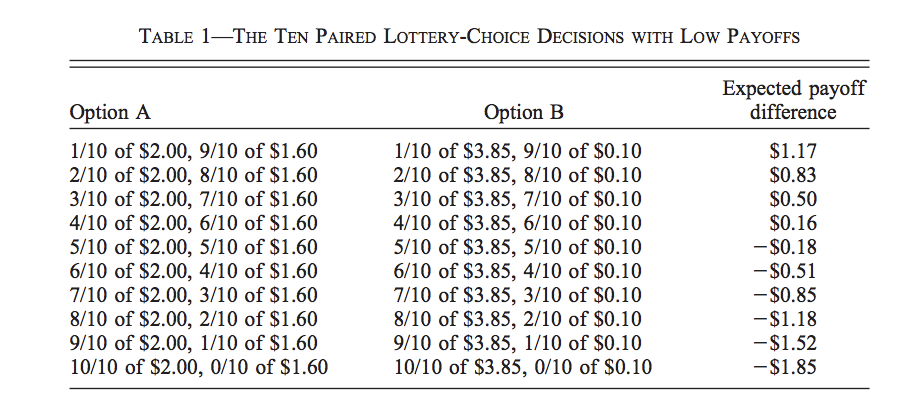
\includegraphics[scale=0.4]{lotteries.png} 
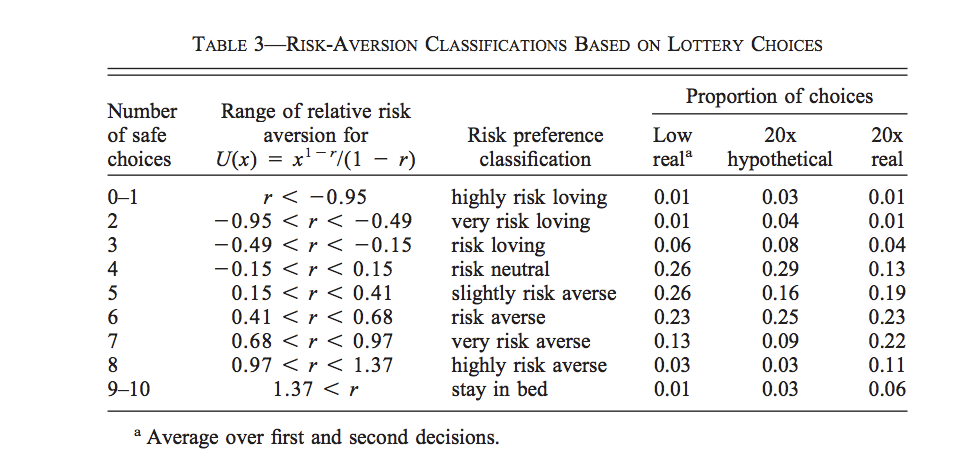
\includegraphics[scale=0.4]{choices.png}
\caption{\href{https://pubs.aeaweb.org/doi/pdfplus/10.1257/000282802762024700}{Holt et Laury (2002), American Economic Review}}
\end{figure}

\textbf{Exercice D}: Pourquoi l'agent averse au risque attend plus longtemps?
\end{frame}

\section{Prime de risque}

\begin{frame}\frametitle{Prime de risque}

\begin{iPar}{Définition} \item Considérons la lotterie $\mc L =
(p,X\;;1-p,Y)$. Définissons $Z$ par $Z \equiv pX+ (1-p)Y$. \item Trouver $Z'$ tel que $u(Z') = pu(X) + (1-p)u(Y)$ \item $Z'$ est l'équivalent certain de $\mc L$ \item Quand riscophobe, $Z' < Z$ et $
\pi = Z-Z'$ est la prime de risque \item La prime est le montant équivalent à ce que la loterie donne de plus (moins) en bien-être \item C'est combien on devrait donner au consommateur pour qu'il prenne ce risque (compensation).
\item Utilisé pour valoriser des actifs risqués
\end{iPar}

\end{frame}

\begin{frame}{Exemple}
\textbf{Exercice E}: Un agent a la fonction d'utilité $u(X)=\log X$. Il a une richesse initiale $X_0 = 100$ et fait façe à un risque de perdre 50 avec probabilité 0.5 et gagner 50 avec probabilité 0.5. Qu'elle est le montant maximum qui est prêt à payer pour éviter le risque?
\textbf{Exercice F}: Avec $u(X) = \sqrt X $, la prime de risque est-t-elle plus faible?
\end{frame}


\section{Applications: Assurance et Investissement}

\begin{frame}\frametitle{Plusieurs des biens qu'on achète sont des lotteries}
\begin{iPar}{Actifs financiers, assurance, biens d'investissement ...
presque tout} \item Actions (paie 10 si la firme performe, paie 0 si elle sous-performe) \item Assurance contre le feu (paie 5 si maison brûle, paie 0
sinon) \item Automobile usagée (valeur de 3 de bonne qualité, valeur de 0 si mauvaise qualité) \item
Se lancer en affaire (paie 15 si fonctionne, paie -5 si on se plante) \item Se marier, choisir une carrière, avoir ou non une chirurgie, conduire un véhicule... sont tous des choix dans un contexte risqué. \end{iPar} \mdp \textbf{Ensuite:} implications pratiques de l'aversion au risque \end{frame}

\begin{frame}\frametitle{Assurance et co-assurance -- I}
\begin{iPar}{Contexte: deux consommateurs face au risque}  \item chacun employé avec probabilité 50\% , revenu 100 \item au chômage (U) avec probabilité 50\%, revenu
0\end{iPar}\mdp

\begin{iPar}{Assurance-emploi} \item Programme d'assurance où
le consommateur 1 en lieu d'obtenir $I_1$ et le consommateur 2 $I_2$ ceux-ci obtiennent $(I_1+I_2)/2$ peu importe leur statut d'emploi \end{iPar}

\end{frame}

\begin{frame} \frametitle{Assurance et co-assurance -- II}

\begin{iPar}{Assurance est bénéfique} \item Sans assurance: 50\%
obtient 0, 50\% obtient 100 \item espérance d'utilité $ .5 [u(0) + u(100)] $ \item
Avec assurance 25 \% obtient 0, 25\% obtient 50, 25\% obtient 50, 25\% obtient
100 \item espérance d'utilité $.25[u(0) + u(50) + u(50) + u(100)]$ \item
Assurance est bénéfice si et seulement si \begin{eqnarray*} & .25[u(0) + u(50) +
u(50) + u(100)] > .5 [u(0) + u(100)]\\ \iff& u(50) > .5[u(0)+u(100)]
\end{eqnarray*}\item Vrai s'ils sont riscophobes  \end{iPar}

\end{frame}

\begin{frame} \frametitle{Assurance et co-assurance -- III}
\begin{iPar}{En pratique} \item Problème si on fait informellement:
ex-ante (avant qu'on connaisse le statut) on veut s'assurer (partager), mais ex-post, si employé, je ne veux plus partager \item Rôle des compagnies d'assurance
(s'assurer que les primes sont payées même s'ils ont été chanceux)\end{iPar}

\end{frame}

\begin{frame} \frametitle{La loi des grands nombres et l'assurance}

\begin{iPar}{Loi des grands nombres} \item Considérons une variable aléatoire $Z$
égale à  $X$ avec probabilité $p$ et $Y$ avec probabilité $1-p$ \item Si $Z_1,
\cdots , Z_n$ sont indépendants avec la même distribution $(p,X \;; 1-p,Y)$
Alors $$si\; N \to +\infty,\quad  \frac{1}{N} (Z_1 + Z_2 + \cdots + Z_n)
\to pX + (1-p)Y$$

\item La moyenne empirique converge sur l'espérance \end{iPar}
\end{frame}


\begin{frame} \frametitle{La loi des grands nombres et l'assurance}

\begin{iPar}{Qu'est-ce que ca veut dire pour l'assurance} \item Quand plusieurs partagent le risque, si tous les risques sont indépendants, alors ils recoivent exactement leur revenu espéré \item Si les individus sont riscophobes, c'est un bon résultat \item Plus il y a des gens qui partagent le risque, plus élevé est le bien-être des gens \item Compagnie d'assurance sont des monopoles naturels... \end{iPar}

\end{frame}

\begin{frame}\frametitle{Assurance est importante: Un exemple d'investissement}
\textbf{Projet d'investissement}\begin{itemize} \item Un individu a une richesse de
9 et peut choisir de rien faire ou utiliser toute sa richesse pour se lancer en affaire avec une loterie $\mc L = (.5,0 \;; .5,25)$ \item Utilité de $u(Z) = \sqrt{Z}$ \item \textbf{Exercice G}: Quel est le rendement espéré? Que choisira-t-il ? \end{itemize}\end{frame}

\begin{frame}\frametitle{Assurance encourage investissement}

\begin{iPar}{Avec assurance} \item Au lieu d'investir seul,
l'entrepreneur peut obtenir du financement de l'ange investisseur qui mettra la moitié du capital contre la moitié du rendement \item L'entrepreneur garde 4.5 avec certitude et obtient la moitié des rendements \item La loterie est maintenant $\mc L' = (.5,4.5 \;; .5,17)$ \item \textbf{Exercice H}: Quel choix fait-il?\end{iPar}

 \end{frame}

\section{Critique de l'espérance d'utilité}



\begin{frame}{Critique de l'espérance d'utilité}
\begin{itemize}
\item Paradoxe d'Allais
\item Paradoxe de d'Ellsberg
\item Kahneman et Tversky
\end{itemize}
\end{frame}


\begin{frame}{Choix}


Un chiffre est tiré entre 0 et 99 avec probabilité 1/100 pour chacun des entiers: 

\begin{table}[H]
\begin{tabular}{lrrr}
\hline \hline
Loteries & 0 & 1-10 & 11-99 \\
$L_1$ & 50 & 50 & 50 \\
$L_2$ & 0 & 250 & 50 \\
\hline \hline 
\end{tabular}
\end{table} 


\end{frame}

\begin{frame}{Choix}

Maintenant faisons un nouveau choix entre

\begin{table}[H]
\begin{tabular}{lrrr}
\hline \hline
Loteries & 0 & 1-10 & 11-99 \\
$L_3$ & 50 & 50 & 0 \\
$L_4$ & 0 & 250 & 0 \\
\hline \hline 
\end{tabular}
\end{table} 

\end{frame}

\begin{frame}{Maurice Allais et son Paradoxe}

\textbf{Exercice H}: Montrez que $L_1 \succ L_2$ et $L_4 \succ L_3$ sont incohérent avec la théorie d'espérance d'utilité. 

\begin{figure}
\centering
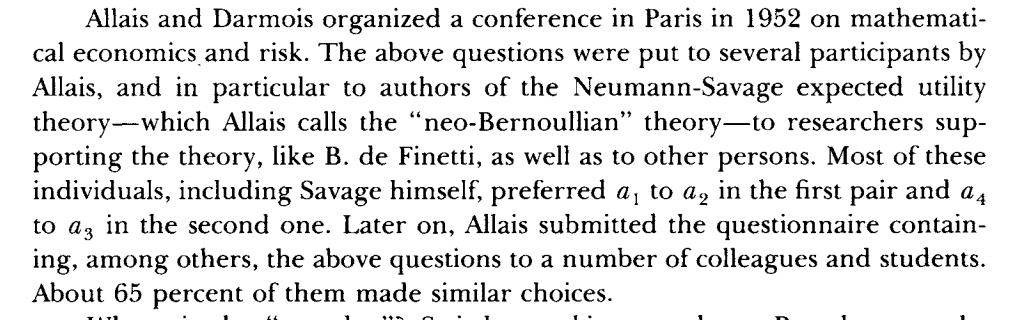
\includegraphics[scale=0.5]{allais.png}
\caption{\href{https://pubs.aeaweb.org/doi/pdf/10.1257/jep.5.2.179}{Munier 1991, Journal of Economic Perspectives}}
\end{figure}

\end{frame}

\begin{frame}{Choix}

Une urne contient 90 billes. 30 sont rouges. Les autres 60 sont noires ou blanches. La proportion des billes noires (et blanches) n'est pas connue. 
Choisir entre
\begin{table}[H]
\begin{tabular}{lrrr}
\hline \hline
Loteries & rouge & noire & blanche \\
$L_1$ & 50 & 0 & 0 \\
$L_2$ & 0 & 50 & 0 \\
\hline \hline 
\end{tabular}
\end{table} 

\end{frame}

\begin{frame}{Choix}

Une urne contient 90 billes. 30 sont rouges. Les autres 60 sont noires ou blanches. La proportion des billes noires (et blanches) n'est pas connue.

\begin{table}[H]
\begin{tabular}{lrrr}
\hline \hline
Loteries & rouge & noire & blanche \\
$L_3$ & 50 & 0 & 50 \\
$L_4$ & 0 & 50 & 50 \\
\hline \hline 
\end{tabular}
\end{table} 
\pause

\end{frame}

\begin{frame}{Paradoxe Ellsberg}

\textbf{Exercice I} Montrez que la combinaison $L_1 \succ L_2$ et $L_4 \succ L_3$ ne respecte pas espérance d'utilité pour toute probabilité subjective de noire. 

\href{https://fr.wikipedia.org/wiki/Daniel_Ellsberg}{Pentagon Papers}

\end{frame}

\begin{frame}{Kahneman et Tversky: Théorie des perspectives}

Imagine new disease, expected to kill 600. Two programs proposed. 

\begin{itemize}
\item (Positive Framing): A) 200 saved, B) 1/3 probability that 600 saved, 2/3 that none saved
\item (Negative Framing): C) 400 will die, D) 1/3 nobody dies, 2/3 all die
	\end{itemize}


Si cela vous intéresse, faut lire: \href{https://www.uzh.ch/cmsssl/suz/dam/jcr:00000000-64a0-5b1c-0000-00003b7ec704/10.05-kahneman-tversky-79.pdf}{Khaneman et Tversky (1979)}

\end{frame}

\end{document}




